  \section{Marco Teórico}
    
Un generador de barrido, puede ser utilizado para obtener la respuesta en frecuencia 
de un amplificador. Para ello el mismo dispone de una salida de señal triangular, que 
se utiliza para realizar el barrido del osciloscopio, y una señal de frecuencia variable 
o de barrido.

Una forma de obtener dicha respuesta, es generar un barrido en frecuencia 
y registrar punto por punto, un esquema que se puede emplear para ello es el que 
se observa en la Figura \ref{fig:GenBarrido}.

\begin{figure}[H]
  \centering
    \frame{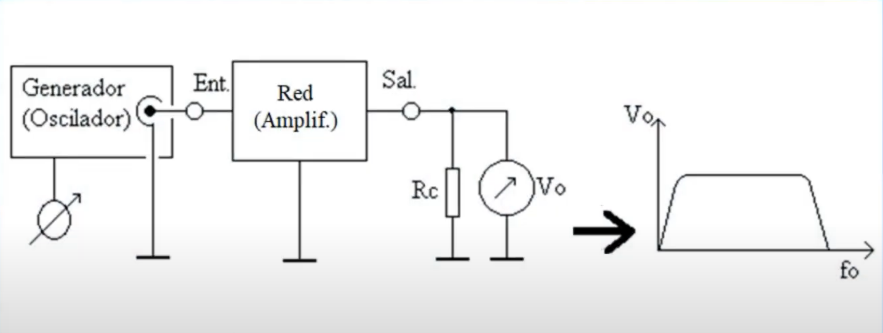
\includegraphics[width=0.6\textwidth]{Imagenes/ActividadPractica/MarcoTeorico/EsquemaGeneradorBarrido.png}}
    \caption{Esquema generador de barrido.}
    \label{fig:GenBarrido}
\end{figure}

Aunque el método propuesto es útil, en la práctica resulta complicado realizar el 
registro de valores. Como solución al problema planteado, se utiliza la señal de barrido para 
el eje horizontal del osciloscopio como muestra la Figura \ref{fig:GenBarridoRed}, que 
permite visualizar de forma automática la respuesta en frecuencia. 

Se puede utilizar el generador en conjunto con un osciloscopio, para simular el 
compartamiento de un analizador de redes.

\begin{figure}[H]
  \centering
    \frame{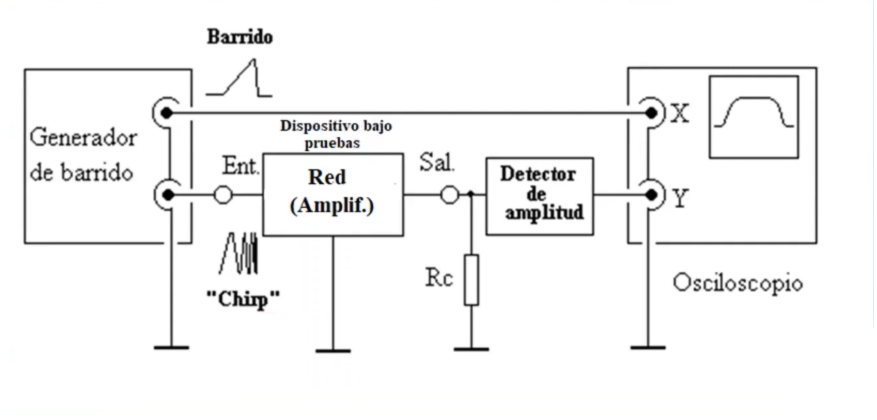
\includegraphics[width=0.6\textwidth]{Imagenes/ActividadPractica/MarcoTeorico/EsquemaGeneradorBarridoYRed.png}}
    \caption{Análisis de red usando un generador de barrido.}
    \label{fig:GenBarridoRed}
\end{figure}

Se logra obtener de ésta manera, la respuesta en frecuencia de una red bajo 
análisis. Sin embargo, 
no es posible conocer con exactitud, la frecuencia a la cual pertenece cada 
medición. Por ésta razón, se hace uso de un generador de marcas.

\begin{figure}[H]
  \centering
    \frame{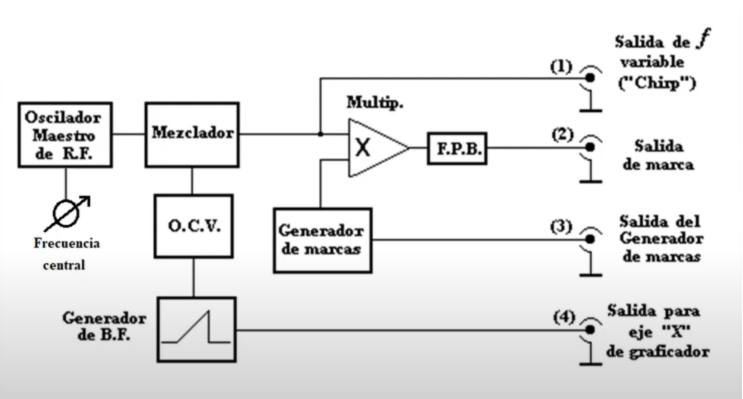
\includegraphics[width=0.6\textwidth]{Imagenes/ActividadPractica/MarcoTeorico/EsquemaGeneradorDeBarridoYMarcas.png}}
    \caption{Esquema de generador de barrido y marcas.}
    \label{fig:GenBarridoYMarca}
\end{figure}

Las salidas del generador de barrido y marcas, se identifican como muestra la Figura \ref{fig:GenBarridoYMarca}.

La salida del modulador se conoce como \textit{PIP}, y es la señal que va a determinar 
la marca visible en el osciloscopio, la cual se genera con lo que se conoce como 
el método del batido cero. 

Luego, se suma la salida del receptor con el PIP y se obtiene la salida del canal vertical.

\begin{figure}[H]
  \centering
    \frame{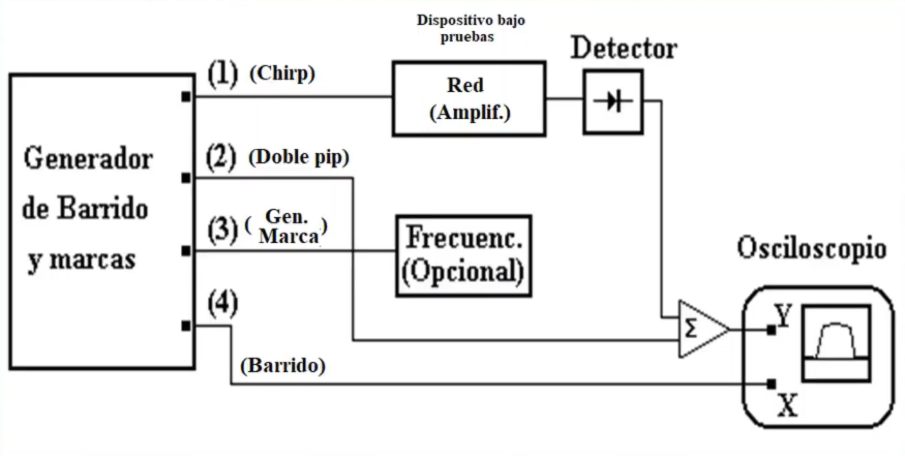
\includegraphics[width=0.6\textwidth]{Imagenes/ActividadPractica/MarcoTeorico/EsquemaGeneradorDeBarridoYMarcasOsciloscopio.png}}
    \caption{Esquema de osciloscopio y generador de barrido y marcas.}
    \label{fig:GenBarridoYMarcaOscilos}
\end{figure}


Los ensayos se realizan en un receptor FM, cuyo esquema simplificado se presenta 
en la Figura \ref{fig:ReceptorSimplificado}. Se presenta a continuación la medición 
que se pretende obtener.

\begin{figure}[H]
  \centering
    \frame{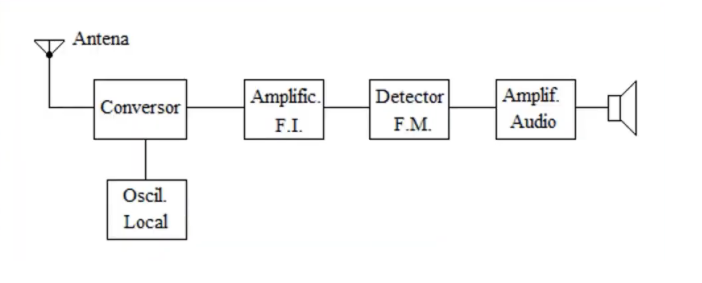
\includegraphics[width=0.6\textwidth]{Imagenes/ActividadPractica/MarcoTeorico/EsquemaSimplificadoReceptorFM.png}}
    \caption{Esquema de Detector FM simplificado.}
    \label{fig:ReceptorSimplificado}
\end{figure}

Se considera como etapa amplificadora, al conjunto formado por el conversor 
y el amplificador, que conforman lo que se denomina \textit{amplificador sintonizado}.

La salida del amplificador se combina con el detector para dar la señal resultante 
a través de la convolución en el tiempo, lo que implica un producto de funciones 
de transferencia en frecuencia. Bajo éste análisis, se deduce la salida del 
receptor de FM, que muestra la Figura \ref{fig:FdeTReceptor}. Dicha salida es de 
utilidad para realizar los ensayos propuestos en el presente informe.

\begin{figure}[H]
  \centering
    \frame{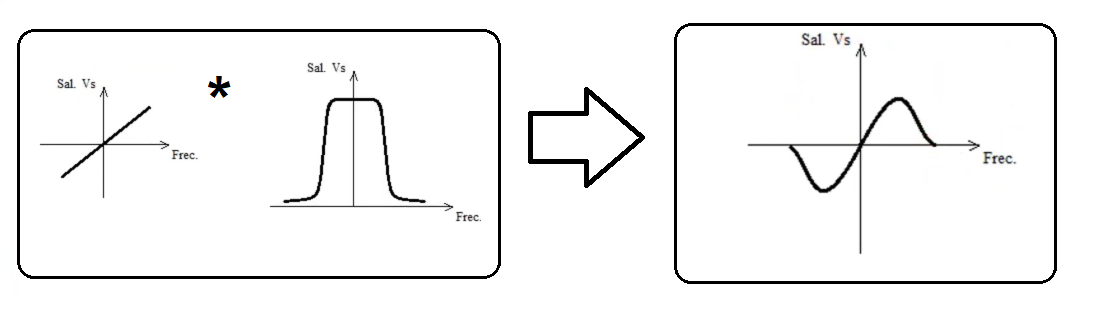
\includegraphics[width=0.6\textwidth]{Imagenes/ActividadPractica/MarcoTeorico/FdeTDetector.png}}
    \caption{Salida del detector.}
    \label{fig:FdeTReceptor}
\end{figure}

